%
\documentclass[11pt]{article}
% Load Packages
%%%%%%%%%%%%%%%%%=
\usepackage[margin=1in]{geometry}
\geometry{letterpaper}
\addtolength{\oddsidemargin}{-0.3in}
\addtolength{\topmargin}{-0.3in}
\addtolength{\textheight}{0.3in}
\addtolength{\evensidemargin}{-0.3in}
\addtolength{\textwidth}{0.6in}
\usepackage{lineno}
\usepackage{enumitem}
%\usepackage{multicol}
\usepackage{fixltx2e}
\usepackage{amsmath,amsfonts,amsthm,amssymb}
\usepackage{graphicx}
\usepackage{tikz,pgfplots}
\usepackage[noend]{algpseudocode}
\usepackage{algorithm,algorithmicx}
\usepackage{url}
\usepackage{color}
\usepackage{varioref}
\usepackage{mathrsfs}
\usepackage[sort&compress,colon,square,numbers]{natbib}
\usepackage{subcaption}
\usepackage[final,authormarkup=none]{changes}
\usepackage{framed}
\usepackage{setspace}
\usepackage{verbatim}
\usepackage{multicol}
\usepackage{dblfloatfix}
\usepackage{wrapfig}
\usepackage{float}
\usepackage{amssymb}
\usepackage{verbatim}
\usepackage{booktabs,colortbl, array}
\usepackage{pgfplotstable,tabularx}
\usepackage{tikz}
\usepackage{pifont}% http://ctan.org/pkg/pifont
\usepackage{caption}
%\usepackage{enumitem}% http://ctan.org/pkg/enumitem
\captionsetup[figure]{font=small}
\captionsetup[table]{font=small}
%\usepackage{enumitem}

%% Set bibliography style
%%%%%%%%%%%%%%%%%%%%%%%%%%%%%%%%%==%%%%%s
%~~

%\renewcommand{\labelenumi}{\Arabic}

%% Declare Colors
%%%%%%%%%%%%%%%%%%%%%%%%%%%%%%%%%%%%%==%

\definecolor{darktangerine}{rgb}{1.0, 0.77, 0.07}
\definecolor{aogr}{rgb}{0.0, 0.5, 0.0}

%% Set Up Checks/Xs

\newcommand{\cmark}{\ding{51}}%
\newcommand{\xmark}{\ding{55}}%
\newcommand{\boldq}{\textbf{?}}

\newcommand{\greencheck}{\textcolor{aogr}\cmark}
\newcommand{\ocheck}{\textcolor{darktangerine}\cmark}
\newcommand{\yellowq}{\textcolor{darktangerine}\boldq}
\newcommand{\redx}{\textcolor{red}\xmark}

%% Set up Tables
%%%%%%%%%%%%%%%%%%%%%%%%%%%%%%%%%%%%%===%
\definecolor{tableheadcolor}{gray}{0.92}
% Following is taken from Werner: http://tex.stackexchange.com/a/33761/3061
% and modified for my needs
%
% Command \topline consists of a (slightly modified)
% \toprule followed by a \heavyrule rule of colour tableheadcolor
% (hence, 2 separate rules)
\newcommand{\topline}{ %
        \arrayrulecolor{MSBlue}\specialrule{0.1em}{\abovetopsep}{0pt}%
        \arrayrulecolor{tableheadcolor}\specialrule{\belowrulesep}{0pt}{0pt}%
        \arrayrulecolor{MSBlue}}
% Command \midline consists of 3 rules (top colour tableheadcolor, middle colour black, bottom colour white)
\newcommand{\midtopline}{ %
        \arrayrulecolor{tableheadcolor}\specialrule{\aboverulesep}{0pt}{0pt}%
        \arrayrulecolor{MSBlue}\specialrule{\lightrulewidth}{0pt}{0pt}%
        \arrayrulecolor{white}\specialrule{\belowrulesep}{0pt}{0pt}%
        \arrayrulecolor{MSBlue}}
% Command \bottomline consists of 2 rules (top colour
\newcommand{\bottomline}{ %
        \arrayrulecolor{white}\specialrule{\aboverulesep}{0pt}{0pt}%
        \arrayrulecolor{MSBlue} %
        \specialrule{\heavyrulewidth}{0pt}{\belowbottomsep}}%


\newcommand{\midheader}[2]{%
        \midrule\topmidheader{#1}{#2}}
\newcommand\topmidheader[2]{\multicolumn{#1}{c}{\textsc{#2}}\\%
                \addlinespace[0.5ex]}

\pgfplotstableset{normal/.style ={%
        header=true,
        string type,
        font=\addfontfeature{Numbers={Monospaced}}\small,
    	column type={p{.092\textwidth}},
        every odd row/.style={
            before row=
        },
        every head row/.style={
            before row={\topline\rowcolor{tableheadcolor}},
            after row={\midtopline}
        },
        every last row/.style={
            after row=\bottomline
        },
        col sep=&,
        row sep=\midrule
    }
}
% Setup Tikz Plots
%%%%%%%%%%%%%%%%%==
\tikzset{
    flowbox/.style={
        rectangle, rounded corners, minimum width=2cm, minimum height=1cm,text centered, draw=black
    },
    stdarrow/.style={->,>=latex, line width=1.5pt}
}
\pgfplotsset{compat=newest}

% Define Some Math Operators
%%%%%%%%%%%%%%%%%%%%%===
\labelformat{equation}{\textup{(#1)}}
\DeclareMathOperator*{\rank}{rank}
\DeclareMathOperator*{\range}{range}
\DeclareMathOperator*{\spn}{span}
\DeclareMathOperator*{\acos}{acos}
\DeclareMathOperator*{\Discriminability}{\textit{Discriminability}}
\DeclareMathOperator*{\iid}{\overset{iid}{\sim}}

% Define custom column widths
%%%%%%%%%%%%%%%%%%%%%%%%%%%%%=
\setlength{\columnsep}{1cm}
%\setlist[enumerate, 1]{label=\textbf{\alph*.}}
\usepackage{array}
%\newcolumntype{L}{>{\raggedright\arraybackslash}m{3.55cm}}
%\newcolumntype{Q}{>{\raggedright\arraybackslash}m{3.35cm}}

% TODOs 
%%%%%===
\newcommand{\todo}[1]{{\color{red}{\it TODO: #1}}}
\newcommand{\greg}[1]{{\color{cyan}{\it greg: #1}}}
\newcommand{\jovo}[1]{{\color{purple}{\it jovo: #1}}}
\newcommand{\eb}[1]{{\color{red}{\it eb: #1}}}

% Shorthand
%%%%%%%%%===
\newcommand{\sic}[0]{{\textsc{SIC}}}
\newcommand{\ndmg}[0]{{\textsc{NDMG}}}
\newcommand{\ndmgd}[0]{{\textsc{NDMG-d}}}
\newcommand{\ndmgf}[0]{{\textsc{NDMG-f}}}



%%%%%%%%% MATH OPERATORS %%%%%%%%%%%%
\providecommand{\ve}[1]{\boldsymbol{#1}}
\providecommand{\ma}[1]{\boldsymbol{#1}}
\providecommand{\norm}[1]{\left \lVert#1 \right  \rVert}
\providecommand{\deter}[1]{\lvert #1 \rvert}
\providecommand{\abs}[1]{\left \lvert #1 \right \rvert}
\providecommand{\mat}[1]{\left[ #1 \right]}
\newcommand{\trans}[1]{{#1}^{\ensuremath{\mathsf{T}}}}           % transpose
\newcommand{\transpose}[1]{{#1}^{\ensuremath{\mathsf{T}}}}           % transpose
\newcommand{\argmax}{\operatornamewithlimits{argmax}}
\newcommand{\argmin}{\operatornamewithlimits{argmin}}
\newcommand{\TT}{^{\ensuremath{\mathsf{T}}}}           % transpose
\newcommand{\from}{{\ensuremath{\colon}}}           % :
\newcommand{\trace}[1]{{\ensuremath{\operatorname{tr}\!\left(#1\right)}}}           % :

\providecommand{\ms}[1]{\mathsf{#1}}
\providecommand{\mc}[1]{\mathcal{#1}}
\providecommand{\mt}[1]{\widetilde{#1}}
\providecommand{\mtt}[1]{\ensuremath{\mathtt{#1}}}
\providecommand{\mb}[1]{\boldsymbol{#1}}
\providecommand{\mbb}[1]{\mathbb{#1}}
\providecommand{\mv}[1]{\vec{#1}}
\providecommand{\mh}[1]{\hat{#1}}
\providecommand{\wh}[1]{\widehat{#1}}
\providecommand{\mhv}[1]{\mh{\mv{#1}}}
\providecommand{\mvh}[1]{\mv{\mh{#1}}}
\providecommand{\mhc}[1]{\hat{\mathcal{#1}}}
\providecommand{\mbc}[1]{\mb{\mathcal{#1}}}
\providecommand{\mvc}[1]{\mv{\mathcal{#1}}}
\providecommand{\mtc}[1]{\widetilde{\mathcal{#1}}}
\providecommand{\mth}[1]{\mt{\mh{#1}}}
\providecommand{\mht}[1]{\mh{\mt{#1}}}
\providecommand{\mhb}[1]{\hat{\boldsymbol{#1}}}
\providecommand{\whb}[1]{\widehat{\boldsymbol{#1}}}
\providecommand{\mvb}[1]{\vec{\boldsymbol{#1}}}
\providecommand{\mtb}[1]{\widetilde{\boldsymbol{#1}}}
\providecommand{\mbt}[1]{\widetilde{\boldsymbol{#1}}}
\providecommand{\mvc}[1]{\vec{\mathcal{#1}}}
% \newcommand{\D}[2]{\frac{\partial #1}{\partial #2}}
\newcommand{\dd}[2]{\frac{\partial ^2 #1}{\partial #2 ^2}}
\newcommand{\DDD}[3]{\frac{\partial ^2 #1}{\partial #2 \partial #3}}
\newcommand{\Di}[2]{\frac{\partial ^i #1}{\partial #2 ^i}}



%%%%%%%%%% ENVIRONMENTS %%%%%%%%%%%%%

\newtheorem{Rem}{Remark}%[section]
\newtheorem{Alg}{Algorithm}%[section]
\newtheorem{thm}{Theorem}
\newtheorem{Thm}{Theorem}[section]
\newtheorem{lem}{Lemma}
\newtheorem{Lem}{Lemma}%[section]
\newtheorem{defi}{Definition}
\newtheorem{Def}{Definition}[section]
\newtheorem{prop}{Proposition}
\newtheorem{coro}[thm]{Corollary}
\newtheorem{claim}{Claim}
\newtheorem{conj}{Conjecture}
\newtheorem{question}{Question}
\newtheorem{answer}{Answer}
\newtheorem{rem}{Remark}%[section]
\newtheorem{cor}[lem]{Corollary}
\newtheorem{model}{Model}
\newtheorem{remark}{Remark}

\newcommand{\bla}{\begin{block}}
\newcommand{\blb}{\end{block}}

\newcommand{\defa}{\begin{defi}}
\newcommand{\defb}{\end{defi}}
\newcommand{\theHalgorithm}{\arabic{algorithm}}

\newcommand{\thma}{\begin{thm}}
\newcommand{\thmb}{\end{thm}}

\newcommand{\mata}{\begin{bmatrix}}
\newcommand{\matb}{\end{bmatrix}}

\floatname{algorithm}{Procedure}
\renewcommand{\algorithmicrequire}{\textbf{Input:}}
\renewcommand{\algorithmicensure}{\textbf{Output:}}
\floatname{algorithm}{Pseudocode}





%%%%%% SHORT HAND %%%%%%%%%%
\renewcommand{\refname}{References and Notes}

\newcommand{\jv}{Joshua Vogelstein}

\newcommand{\Vr}{V_{reset}}
\newcommand{\Vl}{V_{leat}}
\newcommand{\eqdef}{\overset{\triangle}{=}}
\newcommand{\grad}{\nabla}
\newcommand{\Hess}{\nabla\nabla}
\newcommand{\defn}{\overset{\triangle}{=}}

\newcommand{\rto}{\leftarrow}
\newcommand{\knn}{$k$NN}

\newcommand{\elegans}{\emph{C. elegans} }

\newcommand{\Lik}{\mathcal{L}}
\newcommand{\Cae}{[\widehat{\text{Ca}}^{2+}]}
\newcommand{\Cav}{\ve{C}}%[\ve{\text{Ca}}^{2+}]}
\newcommand{\sml}{\sqrt{\ma{\lambda}}}
\newcommand{\ml}{\ma{\lambda}}
\newcommand{\nw}{\widehat{n}}
\newcommand{\nv}{\vec{n}}
\newcommand{\Ae}{\widehat{A}}
\newcommand{\te}{\widehat{\tau}}
\newcommand{\maxn}{\max_{\ve{n}: n_t \geq 0}}
% \newcommand{\V}{\text{Var}}

\newcommand{\PmcP}{P \in \mc{P}}
\newcommand{\mP}{\mathbb{P}}

% \newcommand{\dvs}{\dot{\bs}_t}
% \newcommand{\dvw}{\dot{\bw}_t}
% \newcommand{\dvx}{\dot{\bx}_t}
% \newcommand{\dvy}{\dot{\by}_t}

\newcommand{\ft}{f_{\ve{\thet}}}
\newcommand{\gt}{g_{\ve{\thet}}}
\newcommand{\hht}{h_{\thetn}}

\newcommand{\Real}{\mathbb{R}}
\newcommand{\Ind}{\mathbb{I}}

\newcommand{\wconv}{\overset{i.p.}{\rightarrow}}
\newcommand{\sconv}{\overset{i.p.}{\rightarrow}}
\newcommand{\conv}{\rightarrow}
\newcommand{\pconv}{\overset{p}{\conv}}
\newcommand{\mcE}{\mathcal{E}}
\newcommand{\mcT}{\mathcal{T}}
\newcommand{\mcG}{\mathcal{G}}
\newcommand{\mcM}{\mathcal{M}}
\newcommand{\mcL}{\mathcal{L}}
\newcommand{\hatmcE}{\widehat{\mcE}}
\newcommand{\hatp}{\widehat{p}}
\newcommand{\hatP}{\widehat{P}}
\newcommand{\hatQ}{\widehat{Q}}
\newcommand{\hatL}{\widehat{L}}
\newcommand{\mhP}{\widehat{\PP}}
\newcommand{\tildeA}{\widetilde{A}}
\newcommand{\defeq}{\overset{\triangle}{=}}


\DeclareMathOperator{\Pmat}{\mathbf{P}}
\DeclareMathOperator{\veta}{\mathbf{\mb{v}}}
\DeclareMathOperator*{\minimize}{\mathrm{minimize}}
\DeclareMathOperator*{\maximize}{\mathrm{maximize}}
% \DeclareMathOperator*{\mb{v}mod}{\mathbf{\mb{v}}}


%%%%%%% LATIN LETTERS


\newcommand{\bA}{\mb{A}}
\newcommand{\bB}{\mb{B}}
\newcommand{\bD}{\mb{D}}
\newcommand{\bE}{\mb{E}}
\newcommand{\bI}{\mb{I}}
\newcommand{\bP}{\mb{P}}
\newcommand{\bS}{\mb{S}}
\newcommand{\bU}{\mb{U}}
\newcommand{\bV}{\mb{V}}
\newcommand{\bW}{\mb{W}}
\newcommand{\bX}{\mb{X}}
\newcommand{\bY}{\mb{Y}}
\newcommand{\bZ}{\mb{Z}}

\newcommand{\ba}{\mb{a}}
\renewcommand{\ba}{\mb{b}}
\newcommand{\bd}{\mb{d}}
\newcommand{\be}{\mb{e}}
\newcommand{\bp}{\mb{p}}
\newcommand{\bs}{\mb{s}}
\newcommand{\bu}{\mb{u}}
\newcommand{\bv}{\mb{v}}
\newcommand{\bw}{\mb{w}}
\newcommand{\bx}{\mb{x}}
\newcommand{\by}{\mb{y}}
\newcommand{\bz}{\mb{z}}


\newcommand{\Aa}{\mathbb{A}}
\newcommand{\BB}{\mathbb{B}}
\newcommand{\CC}{\mathbb{C}}
\newcommand{\DD}{\mathbb{D}}
\newcommand{\EE}{\mathbb{E}}           % expected value
\newcommand{\FF}{\mathbb{F}}
\newcommand{\GG}{c}
\newcommand{\HH}{\mathbb{H}}
\newcommand{\II}{\mathbb{I}}           % indicator function
\newcommand{\LL}{\mathbb{L}}
\newcommand{\MM}{\mathbb{M}}
\newcommand{\NN}{\mathbb{N}}
\newcommand{\PP}{\mathbb{P}}
\newcommand{\QQ}{\mathbb{Q}}
\newcommand{\SSS}{\mathbb{S}}
\newcommand{\VV}{\mathbb{V}}
\newcommand{\WW}{\mathbb{W}}
\newcommand{\XX}{\mathbb{X}}
\newcommand{\YY}{\mathbb{Y}}
\newcommand{\ZZ}{\mathbb{Z}}




\newcommand{\Qs}{Q}
\newcommand{\mcS}{\mc{S}}
\newcommand{\mcU}{\mc{U}}

\newcommand{\mbd}{\ensuremath{\mb{d}}}
\newcommand{\mbD}{\ensuremath{\mb{D}}}
\newcommand{\mbx}{\ensuremath{X}}
\newcommand{\mbX}{\ensuremath{\mb{X}}}
\newcommand{\mby}{\ensuremath{Y}}
\newcommand{\mbY}{\ensuremath{\mb{Y}}}

\newcommand{\mtbd}{\mtb{d}}
\newcommand{\mtbD}{\mtb{D}}
\newcommand{\mtbx}{\mtb{x}}
\newcommand{\mtbX}{\mtb{X}}
\newcommand{\mtby}{\mtb{y}}
\newcommand{\mtbY}{\mtb{Y}}



\DeclareMathOperator{\Ri}{\mathbf{\R}^{-1}}
\DeclareMathOperator{\A}{A}
\DeclareMathOperator{\W}{\mathbf{W}}
\DeclareMathOperator{\V}{\mathbf{V}}
%\DeclareMathOperator{\U}{\mathbf{U}}
%\DeclareMathOperator{\C}{\mathbf{C}}
\DeclareMathOperator{\uvec}{\mathbf{u}}
\DeclareMathOperator{\D}{\mathbf{D}}
\DeclareMathOperator{\Q}{\mathbf{Q}}
\DeclareMathOperator{\R}{R} %\mathbf{P}}
\DeclareMathOperator{\Y}{\mathbf{Y}}
%\DeclareMathOperator{\BB}{\mathbf{B}}
\DeclareMathOperator{\Hmat}{\mathbf{H}}
\DeclareMathOperator{\Gmat}{\mathbf{G}}
\DeclareMathOperator{\X}{\mathbf{X}}
\DeclareMathOperator{\Cmat}{C} %\mathbf{L}}\providecommand{\ms}[1]{\mathsf{#1}}

\DeclareMathOperator*{\Ymod}{\mathbf{\Y}}
\DeclareMathOperator*{\Bmod}{\mathbf{B}}
\DeclareMathOperator*{\Hmod}{\mathbf{H}}
\DeclareMathOperator*{\Lmod}{\mathbf{L}}
\DeclareMathOperator*{\Xmod}{\mathbf{\X}}


%%% THETA %%%%

\newcommand{\bth}{\ve{\theta}}
\newcommand{\hth}{\mh{\theta}}
\newcommand{\htth}{\mh{\theta}}
\newcommand{\bhth}{\mh{\ve{\theta}}}
\newcommand{\thetn}{\ve{\theta}}
\newcommand{\thet}{\thetn}
\newcommand{\theth}{\widehat{\ve{\theta}}}
\newcommand{\theto}{\ve{\theta}'}
\newcommand{\wht}{\widehat{\thet}}
\newcommand{\wtt}{\widetilde{\thet}}
\newcommand{\vth}{\ve{\thet}}
\newcommand{\vTh}{\ve{\Theta}}
\newcommand{\hvth}{\widehat{\ve{\thet}}}
\newcommand{\bTh}{\ve{\Theta}}
\newcommand{\hbth}{\widehat{\thet}}
\newcommand{\tbth}{\tilde{\bth}}



% \newcommand{\p}{P_{\bth}}
\newcommand{\pold}{P_{\bth'}}
\newcommand{\pk}{P_{\widehat{\ve{\theta}}^{(k)}}}
\newcommand{\pT}{P_{\thetn_{Tr}}} %\thetn_T
\newcommand{\pO}{P_{\thetn_o}} %\thetn_o
% \newcommand{\Q}{Q(\thetn,\theto)}
% \newcommand{\m}{m^{\ast}}
% \newcommand{\q}{q(\ve{H}_t)}
\newcommand{\Ca}{[\text{Ca}^{2+}]}


%%%%%% GREEK LETTERS

\newcommand{\del}{\delta}
\newcommand{\sig}{\sigma}
\newcommand{\lam}{\lambda}
\newcommand{\gam}{\gamma}
\newcommand{\eps}{\varepsilon}

\newcommand{\Del}{\Delta}
\newcommand{\Sig}{\Sigma}
\newcommand{\Lam}{\Lambda}
\newcommand{\Gam}{\Gamma}

\newcommand{\bSig}{\ve{\Sigma}}
\newcommand{\bOm}{\ve{\Omega}}
\newcommand{\bLam}{\ve{\Lambda}}
\newcommand{\bPhi}{\ve{\Phi}}
\newcommand{\bPsi}{\ve{\Psi}}

\newcommand{\bmu}{\ve{\mu}}
\newcommand{\bal}{\ve{\alpha}}
\newcommand{\bpi}{\ve{\pi}}
\newcommand{\bkap}{\ve{\kappa}}
\newcommand{\bdel}{\ve{\delta}}
\newcommand{\bphi}{\ve{\phi}}
\newcommand{\bpsi}{\ve{\psi}}



\DeclareMathOperator{\Delti}{\mathbf{\Delta}^{-1}}
\DeclareMathOperator{\Delt}{Q} %\mathbf{\Delta}}
% \DeclareMathOperator{\Gam}{\mathbf{\Gamma}}
\DeclareMathOperator{\Gami}{\mathbf{\Gamma}^{-1}}
\DeclareMathOperator{\Sigb}{\mathbf{\Sigma}}






%%%%%%%%%%% ALGORITHM NAMES %%%%%%%%%%%%%

%\providecommand{\sct}[1]{{\sc \texttt{#1}}}

\providecommand{\sct}[1]{{\sc \texttt{#1}}}

\newcommand{\Idt}{\sct{Idt}}
\newcommand{\Svd}{\sct{Svd}}
\newcommand{\Pca}{\sct{Pca}}
\newcommand{\Fld}{\sct{Fld}}
\newcommand{\Lda}{\sct{Lda}}
\newcommand{\eig}{\sct{eig}}
\newcommand{\Lol}{\sct{Lol}}
\newcommand{\Lal}{\sct{Lal}}
\newcommand{\Qoq}{\sct{Qoq}}
\newcommand{\Lrl}{\sct{Lrl}}
\newcommand{\Lfl}{\sct{Lfl}}
\newcommand{\Faq}{\sct{Faq}}
\newcommand{\qr}{\sct{qr}}

\newcommand{\Mgc}{\sct{Mgc}}
\newcommand{\Mgcp}{\Mgc$_P$}
\newcommand{\Mgcd}{\Mgc$_D$}
\newcommand{\Mgcm}{\Mgc$_M$}
\newcommand{\Hhg}{\sct{Hhg}}
\newcommand{\Dcorr}{\sct{Dcorr}}
\newcommand{\Dcov}{\sct{Dcov}}
\newcommand{\Mcorr}{\sct{Mcorr}}
\newcommand{\Mantel}{\sct{Mantel}}
\newcommand{\Mic}{\sct{Mic}}
\newcommand{\Hsic}{\sct{Hsic}}
\newcommand{\Pearson}{\sct{Pearson}}
\newcommand{\Kendall}{\sct{Kendall}}
\newcommand{\Spearman}{\sct{Spearman}}
\newcommand{\RV}{\sct{RV}}
\newcommand{\CCA}{\sct{Cca}}

\usepackage{neurodata}


\title{What is Connectome Coding?
}
% Statistical versus Statisticlish Connectomics
% title game on point. definitely a keeper :) -eb

\begin{document}

\maketitle
\noindent\parbox{0.9\textwidth}{
\normalsize\color{lgray} Joshua T.~Vogelstein$^1$ (\url{jovo@jhu.edu}),
Eric W.~Bridgeford$^1$, 
% Daniel Sussman$^2$, 
% Vince Lyzinski$^3$, 
% Yichen Qin$^4$, 
% Youngser Park$^1$, 
Brett Mensh$^5$, 
% Brian Caffo$^1$, 
Carey E. ~Priebe$^1$, 
% , $\sigma$(heather, martin,  avanti, minh, dpmcsuss, yichen) 
\\
$^1$ Johns Hopkins University, $^2$ Boston University, $^3$ University of Massachusetts, Amherst, \\ $^4$ University of Cincinnati, $^5$ Janelia Research Campus
}
\thispagestyle{empty}
\medskip
\vspace{10pt}


\noindent
% @BM: write a 3 sentence abstract.
\textbf{TBD
% Analogous to the neural code, which is a model that characterizes the relationships between brain activity and sensory input and motor output, the connectome code is a model that  characterizes the  relationship  between brain  structure and brain or body  activities, encoded in either plasticity or development. 
% We describe the basic statistical formulation and motivation for the connectome code, while  providing a number  of examples across the phylogenetic spectrum as well as  experimental modalities spanning spatiotemporal scales.  Connectome coding is an emerging sub-discipline in neuroscience with many open opportunities.
}


%\begin{multicols}{2}


\section{A Conceptual Model of Brains, Bodies, and Worlds}
% @BM: spandrels?
% @BM: different ways of doing science: data "speaks for itself" and we have super simple conceptual models, vs needing complex statistical modeling. science is always both things, people pretend that they think of an idea, and then generate the data, etc.  
% @BM: hey connectomists: consider evolution guides development of connectomes, and connectomes drive behavior. also, people studying activity, recall connectomes are required for mechanisms.
% @BM: give examples, but all existing examples are either too simple or too coarse to be interesting.



\begin{wrapfigure}{r}{0.5\textwidth}
  \begin{center}
    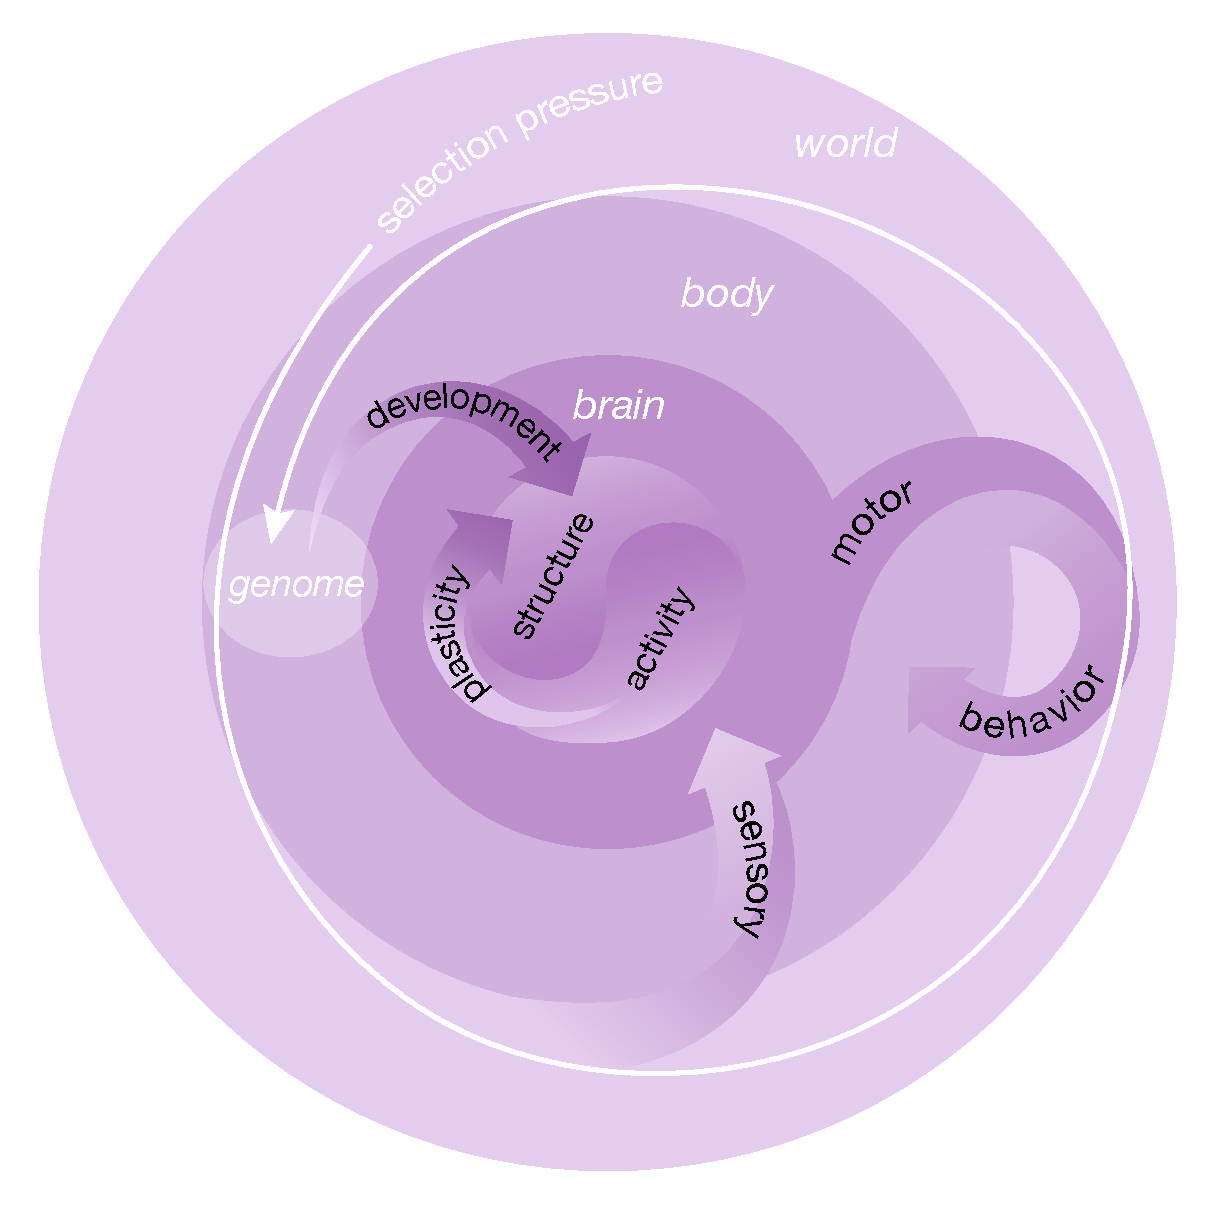
\includegraphics[width=0.48\textwidth]{figs/brain-body-world.pdf}
  \end{center}
  \caption{TBD
%   The connectome code is a model characterizing how information from brain activity and the genome is represented in the brain by connections between morphological objects (the connectome),  and how that brain  structure  in  turn impacts  brain activity and by it, motor control, behavior, and eventually evoluationary fitness.
  }
	\label{f:code}
\end{wrapfigure}

In this article we propose a quantitative modeling framework to characterize and explain certain aspects of brain structure.  Any quantitative modeling framework either implicitly or explicitly rests on a conceptual model. While our conceptual model is not entirely novel, making it explicit reveals certain inadequacies of the existing neuroscience modeling frameworks and tools, thereby motivating the development on the strategy proposed below.

In our conceptual model, there are three ``levels'' of physical objects: a brain, a body, and a world (Figure~\ref{f:code}).  Each level exhibits both internal dynamics and interacts across levels.  These interactions occur across many orders of magnitude of both space and time.  
Our main interest is in modeling the brain, and in particular, brain structure, as will be seen below.

Starting from the outer level, the world governs the outcomes of the ongoing evolutionary games within various ecological niches.  In these games, the brain and body must conspire together to behave in ways that out-compete other brains and bodies for shared limited resources.  The body is the source of motor control, as well as sensory input to the brain.  It is therefore the required interface between the brain and the world.  And the brain is further divided into structure (for example, neurons and glia) and activity (for example, dynamics of ions, neurotransmitters, and second messengers).  

From this perspective, it is clear that brain structure plays an integral role in brain activity, motor control, behavior, and eventually the outcomes of evolutionary pressures~\cite{Ramon_y_Cajal1995-sf}. 
In particular, brain structure governs motor sequences in a variety of ways.  For example, a particular brain structure controls the suppresive hierarchy among competing motor programs that drives sequential grooming in Drosophila~\cite{Seeds2014-jp}.  
Similarly, the interscutularis neuromuscular circuit  controls the mouse's ear movements~\cite{Lu2009-us}.  
In both cases, the brain structure must provide a foundation, as well as a set of constraints and biases, that guide brain activity.  
Thus, ``understanding'' the mechanism of those behaviors requires a model of brain structure.  

That a model of brain structure is required to explain the brain's output motivates the search for a model that explains brain structure itself.  
Brain structure is guided  be two components.  First, developmental programs, which are encoded in the genome~\cite{Purves1985-lw}.  Of course, the genome is partially determined by selective pressures imposed on previous generations, where some of the individuals were able to propagate their genes by choosing specific behaviors (and luck)~\cite{Tomasetti2015-wl}.  Second, by activity dependent plasticity, which is encoded in the rules governing, for example, spike-timing-dependent plasticity~\cite{Dan2006-lg}. 
Development and activity dependent plasticity are not fully independent, rather, much of development (and degeneration) is gated or guided by activity, for example, the onset of critical periods~\cite{Scott1962-rv}. 


\section{What is a Connectome?}


A connectome is typically defined as a network, the ``$W_{ij}$'', of the brain of the brain~\cite{Sporns2005-mg, Hagmann2005-ss}.
Recall that a network, in graph theory, consists of a set of nodes and edges connecting them.  In such a network, there is no physical space, no location, no connection strength, etc.  
Thus, a network, as defined by graph theory,  is a bit limiting and overly simplistic for the kinds of analysis and models that people are using to study connectomics.  
Here, we introduce a more general definition of a connectome, which includes (potentially multiscale)   structural attributes, many of which are implicitly included in previous notions of a connnectome.
Any brain network consists of nodes (also called vertices or actors) and edges (also called links or arcs).  
In brain networks, however, nodes are always spatially contiguous morphological objects, whose extent and shape are determined by the spatiotemporal resolution of the experimental modality providing connectome data.  For example, in nanoscale electron microscopy data, the nodes are typically individual neurons, whereas in macroscale magnetic resonance imaging data, nodes may be defined by sulcul and gyral delineations.
Thus, these nodes always have attributes, including absolute location in the brain, often including relative position in a template brain, an associated shape, thickness for cortical areas, branching morphology, and frequently have an associated  hierarchical ontology, of neuron types~\cite{Hodge2018-dr}  or regions~\cite{Hagmann2008-ml, Mai2007-wq}.
Similarly, the edges in nanoscale data can be either chemical or electrical synapses, whereas edges in macroscale data can be defined by correlations over brief epochs of time, or large bundles of axons. 
These edges therefore have a number of attributes, potentially including strength, size, sign, and more.   Therefore, to answer the questions of interest requires a generalized notion of a network or graph, one that includes potentially complex vertex and edge attributes. In summary, we characterize the entirety of the brain structure at a particular scale as the ``connectome'' of that region. 




\subsection{Example Connectomes}
\label{s:examples}

We describe several different estimates of connectomes spanning the phylogenetic tree and spatiotemporal scales.  We will use these connectomes as working examples  to illustrate the power and flexibility of our proposed connectome coding framework. Figure~\ref{f:connectomes} shows adjacency matrices for each of the connectomes.

\textbf{(A) Caenorhabditis elegans}
% \begin{enumerate}[label=\Alph*]
% 	\item 
	The  \emph{Caenorhabditis elegans} (C.~elegans) is the only animal that we have a complete, neuron-to-neuron level connectome. In the C.~elegans connectome, edges are either chemical synapses or gap junctions.  Each edge's strength or weight corresponds to the number of synapses between its parent neurons. There are two sexes of C.~elegans, the male and hermaphrodite, with different numbers of neurons (the male has more, most of the neurons are shared between the two sexes, but not all).  
    %Thus , each sex has a weighted, partially directed, multi-connectome.  
    These connectome estimates  are derived by cumbersome manual tracing of axons and dendrites, and identification of synapses, in nanoscale electron micrographs~\cite{White1986-rd}, and were updated by ~\citet{Varshney2011-rc} and~\cite{Bentley2016-jy}. 
    The neurons are  often divided into  three classes: sensory (S), internal (I), and motor (M), most of which are bilaterally symmetric, though not all the motor neurons have lateral counterparts. 
    Figure~\ref{f:connectomes}(B) shows the hermaphrodite weighted multiconnectome, including both chemical (gray) and electrical (red)  synapses.  Note that chemical synapses are directional, whereas electrical synapses are bidirectional, so the red adjacency matrix is symmetric.
    % (Figure~\ref{f:connectomes}(A)).
    % 
    
% 	\item 
	\textbf{(B) Drosophila melanogaster}
	Eichler et al.~\cite{Eichler2017-yi} published a complete larval Drosophila connectome of both the left and right mushroom body, also derived from serial electron microscopy, using only chemical synapses. These edges are weighted (based on  counting the  number of synapses between a pair of neurons), and  directed.
	Neurons are categorized  into  kenyon cells (K), input neurons (I), output neurons (O), and projection neurons (P).  Figure~\ref{f:connectomes}(B) shows the left mushroom body.
% 	, which  is weighted  and  directed.
%	\item The mouse microscale connectome from the Allen Institute was estimated using light microscopy tracer studies averaging $\approx 1000$ brains~\cite{Oh2014}. The nodes of this network are neuroanatomical regions based on the Allen Reference Atlas  ontology. The resulting network is a directed and weighted network,  where the weight from region $u$ to $v$ correspond to the number of fluorescent voxels in region $v$ whose source neurons are in region $u$, normalized by the size of region $u$ (Figure \ref{f:connectomes}(B)).

    % \item 
    \textbf{(C) Mus musculus}
    Calabrese et al.~\cite{Calabrese2015-gw} generated a high-resolution connectivity estimate using ex vivo diffusion magnetic resonance imaging (dMRI).  This network is undirected, as dMRI lacks directional information, and weights correspond to the number of tracts estimated to go from one region to another. Because we do not know the mapping between  the absolute magnitude of  connection weights to any  physical connection, we rescale these weights to be between zero and one, and depict them in Figure~\ref{f:connectomes}(C) on a log scale.
    Regions in the mouse  connectome can  be  partitioned into ``superstructures'', including frontal (F), hindbrain (H), midbrain (M), and white matter (W).
     
    % \item 
    \textbf{(D) Homo sapiens}
    The Consortium for Reliability and Reproducibility~\cite{Zuo2014-sh} collects multiple measurements of functional resting-state (F),  anatomical (A),  and/or diffusion (D) magnetic resonance imaging per individual (FAD-MRI). The  functional connectomes are Pearson correlation matrices, which have been thresholded, converted to ranks, and then normalized between zero and one,  because such a representation has been shown to be more reliable than raw or thresholded correlations~\cite{reliability}.  The diffussion connectomes are normalized as described above for the mouse. 
    We analyze the multi-connectomes including both functional and diffusion derived estimates derived from averaging the entire dataset consisting of 3,067 dMRI and 1,760 fMRI connectomes~\cite{Kiar2018-bo}. 
    %
    Of the many possible brain parcellations~\cite{Glasser2016-ap}, we elected to  use the Desikan parellation~\cite{desikan}, assigning each cortical region into lobes including frontal (F),  occiptal (O), parietal (P), and temporal (T), as well as sub-cortical structures (S)  (Figure \ref{f:connectomes}(D)).
% \end{enumerate}


\begin{figure}
	\begin{center}\includegraphics[width=0.8\linewidth]{figs/fig_connectomes.pdf}\end{center}
	\caption{\textbf{(A) - (D)} Connectomes spanning four levels of the phylogenetic tree, each acquired using different experimental modalities and spatial resolutions, ranging from nanoscale (electron microscopy) to macroscale (MRI regions).  In each case, the connectomes are depicted as weighted adjacency matrices; for the worm and human, the connectomes are multi-connectomes, with two different edge types, denoted by two different colors. In each case, the vertices are sorted by region.  Moreover, along each connectome we provide the degree sequence, that is, the ``degree centrality'' for each node and modality~\cite{Zuo2012-gm}. \textbf{(E)} Density estimates of the non-zero edge weights per-connectome. The annotated line on each density estimate indicates the average non-zero edge-weight. The fly mushroom body, a binary graph, is not shown as all non-zero edges have weight 1. \textbf{(F)} The fraction of edges per-connectome that are non-zero. The connectomes display sizable disparity in both non-zero edge weight and fraction of non-zero edges.}
	\label{f:connectomes}
\end{figure}
% @EB: consider adding the following:
% 1. updating C. elegans with newer data
% 2. adding male c elegans
% 3. adding other drosophila dataset
% 4. add region labels to x- and y-axes
% 5. make degree distributions conditional, eg, on type, or hemisphere, etc.?
% 6. update drosophila to have both left and right (in red and black), and make  both weighted.
% 7.  ideally, update mouse to also include Allan connectivity.
% 8. i think our plot of nnz vs avg weight makes sense if we restrict it to all the human multigraphs?




\section{What are the Guiding Questions for Studying Connectomics?}



The basic questions concerning connectomes emerge immediately from the conceptual model outlined above.  First, how does a connectome impose constraints and biases on brain activity to guide decision making, motor planning of the body, and behavior in the world, to increase the chances that the organism will be able to propagate its genes to the next generations?  Second, how do the genome, rules of plasticity, and past brain activity shape the connectome to enable the capabilities eluded to in the previous question?  These two questions operate on completely different temporal zones. The first question is about how the connectome impacts the future, the second question is about how the past impacts the connectome.  Because evolution is a spiral trajectory, where the future continuously becomes the past, these two questions are inextricably linked.  In our opinion, satisfactory answers to the questions are quantitative, and will result from careful data analysis and modeling of existing and future connectome data. After introducing our proposed framework, we will formally restate these questions in the language of the proposed framework.



\section{What Properties do we desire for our Quantitative Modeling Framework?}

The key requirement of any framework one would use to begin answering these questions, of course, is that it is ``\emph{sufficient}'' to answer them.  This means that the framework must be able to represent graphs with complex vertex and edge attributes.  
Second, the connectomes on which the framework will operate are fundamentally noisy, the measurements are noisy, and probably the actual connection probabilities in the brain are stochastic.  For example, even a identical twins, or clones, are unlikely to have identical connectomes at all scales.  
This means that the modeling framework must incorporate and \emph{quantify uncertainty}. 
Third, the latent geometric and topological structures that guide the development of connectomes, and that guide the activity given connectomes, could be arbitrarily complex.  The modeling framework should be able to discover such latent properties.
Fourth, that the modeling framework incorporates uncertainty implies the existence of parameters with unknown values, that we desire to estimate from the observed data.
Thus, the modeling framework must be able to provide theoretical guarantees about the ``validity'' and/or ``correctness'' of the parameter and uncertainty estimates, given sufficient data, under the assumed model. In other words, if one desires to estimate the average connectome from a population, and the estimator of the average may or may not converge to the truth, why would one trust that estimate~\cite{Tang2016-conn}. 
Estimators with this property are called ``\emph{consistent}'' in the statistics literature~\cite{Bickel2000-kb}.
Fifth, standard consistent results imply that the estimators converge under certain model assumptions.  However, ``all models are wrong'', which means that we also desire that our estimators perform well despite model uncertainties; in other words, that our estimators are \emph{robust}.
Sixth, using this model to make inferences must be computationally tractable, or better yet, \emph{computationally efficient} (for example, polynomial computing time).  Graph theoretic problems are notorious computationally difficult~\cite{Lyzinski2016-hb}.  Thus, for many questions, either analytic or numeric approximations are necessary to obtain polynomial (rather than exponential) time algorithms.  
We desire that despite those approximations, estimates preserve their consistency properties.  








\section{Can existing frameworks solve connectome coding?}

% \begin{enumerate}
    % \item  
    \textbf{Graph Theory}: Graph theory has recently been promoted as a framework for elucidating connectome codes.  However, the objects under study in graph theory lack attributes.  Specifically, nodes are not named or identified (as a particular neuron or region, for example).  In other words, using a purely graph theoretic analysis, it is literally impossible to differentiate between two connectomes that are topologically identical, even if one completely lacks connections between visual and motor areas, whereas the other lacks connections between auditory and motor areas. In other words, it fails the ``sufficiency'' criterion.  That is not to say that graph theory is not a fantastic foundation upon which one can extend, rather, on its own, it is insufficient. 
    % \item  
    
    \textbf{Bag of Edges}: Another strategy, previously referred to as the ``bag of edges'' approach~\cite{Craddock2013-gf} do not address dependence structure adequately, leads to invalid inferences, p-values, confidence intervals.
    
    
     The simplest approach to compare graphs is to
treat them as a bag, or collection, of edges and perform statistical
analyses at each edge one at a time, without taking into account
interactions or relationships between them (that is, edgewise
statistics)84. Such univariate approaches (for example, t-tests,
F-tests or regression) allow researchers to identify easily interpretable
relationships between categorical or dimensional variables
and edge weights. However, this approach results in the
need to perform many statistical tests, which require correction
for multiple comparisons to adequately control for the number
of false positives. Standard correction techniques such as false
discovery rate86 that do not model the dependencies between
edges may result in overly liberal or conservative corrections87.
Alternate correction techniques such as the network-based statistic88
or group Benjamini-Hochberg89 leverage information about
the group structure of connectome graphs to increase statistical
power, while maintaining control of false positives.
Alternatively, multivariate regression and classification techniques
evaluate the relationship between the entire connectome
graphs and their associated phenotypic variables with a single
statistical test90,91. Although powerful for the analysis of connectome-phenotype
relationships, they obscure information about
the involvement of individual edges. Extracting this information,
if desired, requires a return to edge-specific tests, and the need for
multiple-comparison correction90. Although these multivariate
techniques tend to be applied to bag-of-edges representations,
which ignore graph structure, they can also be performed using
graph-distance measures that preserve topological information
when comparing graphs92.

    % \item 
    
    \textbf{Bag of Features}: ERGM, control theory, etc.
% \end{enumerate}




\section{Why Connectome Coding?}

Interest in studying the  neural code is well-established, despite widespread disagreement about whether there is a single neural code, or one code per problem per species, or per region, or per behavior, etc.  
On the other hand, whether a connectome code is valuable is hotly debated.  Here we outline a few basic reasons that connectome codes are not just valuable, but actually required for a comprehensive understanding of brain function and dysfunction.  
% 
\begin{itemize}
\item It is widely conjectured that information in the brain is stored in neural circuits, also called the memory engram~\cite{Strength2003-yq}. To the extent that this is true, our ability to understand and ``read'' memories will depend on the depth of our understanding of the statistics of these circuits.  
% 
\item Another relatively widely held belief is that psychiatric illnesses are disorders of neural circuitry, or connectopathies~\cite{Castellanos2013-xq, Van_Dam2017-cv, Spronk2018-ph, Elliott2018-bj, Powell2018-ad, Braun2018-cg}. If true, our ability to develop clinically useful prognostic, diagnostic, and treatment protocols will also depend on our understanding of neural circuitry.  In both cases, it remains an open question as to the required ``precision'' of the connectome code.  For example, the degree to which a  neuron,  cell-type, or a region of interest level connectome code will be useful for clinical practice remains an open empirical question.
% 
\item  Neural activity depends on  neural connectivity~\cite{Mill2017-aa}.  The requisite additional information to create a sufficiently biofidelic simulation of a brain continues to be debated,  but all simulations use some connectomic information~\cite{Markram2015-fs}.
\item Finally, in the human brain, there are approximately $10^{11}$ neurons~\cite{Herculano-Houzel2009-zv} and $10^{15}$ connections between pairs of neurons, and yet we only have about $3 \times 10^4$ genes~\cite{Ezkurdia2014-ta}.  This means that the genome must genetically encode the ``blueprint'' of the brain, that is, a number of statistical rules governing the probability of synapses between regions throughout development, as well as all the rules for learning new connections due to activity-dependent plasticity.  
% Thus, evolution must have learned a connectome code for humans, one that we should be able to learn from data.  
\end{itemize}

The above arguments motivate building statistical models for connectome coding, but why can we not simply use the models developed for neural coding?
There are two key differences between connectome coding and neural coding that make connectome coding substantially more difficult. 
First, a spike can be modeled as a function of only a single neuron or node, whereas an edge is fundamentally a function of two nodes.  This complicates matters because even the simplest connectome models become bilinear (linear in both nodes) versus linear (linear in one node).  Bilinearity increases the difficulty of estimating parameters, both computationally and statistically. Second, spikes are fundamentally binary operations: a spiking neuron either spikes or does not, to convey information to downstream neurons.  However, connections between nodes are not binary.  Even individual synapses can vary dramatically in volume and the maximum magnitude of an average evoked potential.  
Estimated connectomes are also typically weighted, whether  they correspond to estimates of the functional or structural relationship between the nodes. Connectomists are therefore faced with a decision: either choose a mechanism for converting weighted networks into binary networks, or develop models for weighted networks.  In either case, this is an additional step not required of those modeling spike trains. 





\section{What is Connectome Coding?}



A code is a system of (potentially stochastic) rules that translate from one representation of information into another.  In  scientific disciplines such as biology, codes are models that  summarize and characterize complex relationships across spatiotemporal resolutions and/or levels of abstraction.  For example, in biology the genetic code is a model describing how sequences of nucleotide triplets are translated into amino acids.  In neuroscience,  ``neural coding'' is a discipline  concerned with translating information to and from \emph{brain activity}, typically  in terms of the spiking activity of neurons (as opposed to  gene expression or glial activity)~\cite{Brown2004-fz}.  
Neural coding seeks to estimate how information is translated (1) \emph{to} current brain activity  from  external  sensory input, and other internal brain activity (such as other neurons firing), 
and (2) from  brain activity into future brain activity, and motor commands that determine  behavior.  


We here introduce another code in neuroscience, the \textbf{connectome code}.  
Connectome coding is a discipline concerned with modeling the translation of information  to and from  \emph{brain  structure}.
Connectome coding seeks to estimate how information is translated (1) \emph{to} brain structure from static and dynamic information  (the somatic genome via development),  and cellular activity and gene expression via   activity dependent plasticity, respectively), and (2) \emph{from} brain structure to activity.
Note that these brain codes model information flow across orders of magnitudes of spatiotemporal scales.  
Evolutionary selective pressures operate across many generations to determine the genome, which encodes for certain coarse connectome properties of phyla.  
For example, the genome of a \emph{Caenorhabditis elegans} (C.~elegans) determines its sex, which causes the presence (or absense) of a subset of neurons.  
Moreover, in nearly all connectomes, bilateral symmetry is encoded (somewhere) in the genome. 
Evolution can also determine macroscale morphological statistical  regularities, such as the number of regions.
% but likely not  specific connections for relatively large connectomes (see below for more details).
Developmental programs operates within a single generation to determine more refined properties of the individual.
For example,  certain developmental mechanisms can go awry leading to various life-long  cognitive disorders~\cite{Karmiloff-Smith2018-ih}.
These can result in mesoscale changes, such as missing corpus callosum~\cite{Paul2007-vy}.
Changes in connections, be they modified strength, or addition/deletion of connections, can happen across minutes, hours, or days, due to  activity-dependent-plasticity~\cite{Carulli2011-pb}. These changes of course happen at a microscale.
Finally, brain activity,  motor output, and sensory input all operate essentially instantaneously.
% 

Figure~\ref{f:code} depicts  a schematic illustrating the different sources of information in brain activity and structure, and how they related to one another via brain codes.  
% 
% Note  that while both neural coding and connectome coding are concerned with  ongoing brain activity, neural coding also considers ongoing sensory stimuli, whereas connectome coding also consider static genomic information.  
% This temporal difference in  coding strategies is key to designing experiments to investigate the different kinds of brain codes. 
% 
Note that both brain activity and structure impact the  behavior of the organism, which in turn is causally related to its fitness, and the evolutionary selective pressures that impact future generations. 
% @BM: the word body does not appear in the intro.

% In both neural coding and  connectome coding, while at one level of abstraction, information is about input and output, at a higher level, is it about behavior and cognition for the survival of the individual, the genes, and the species.  
% @BM: but what actual information? and here’s the biology this whole thing is sorely missing: it is information about how to win, given the game the animal is playing and the body it’s playing it in.



%\begin{figure*}[h!]
%	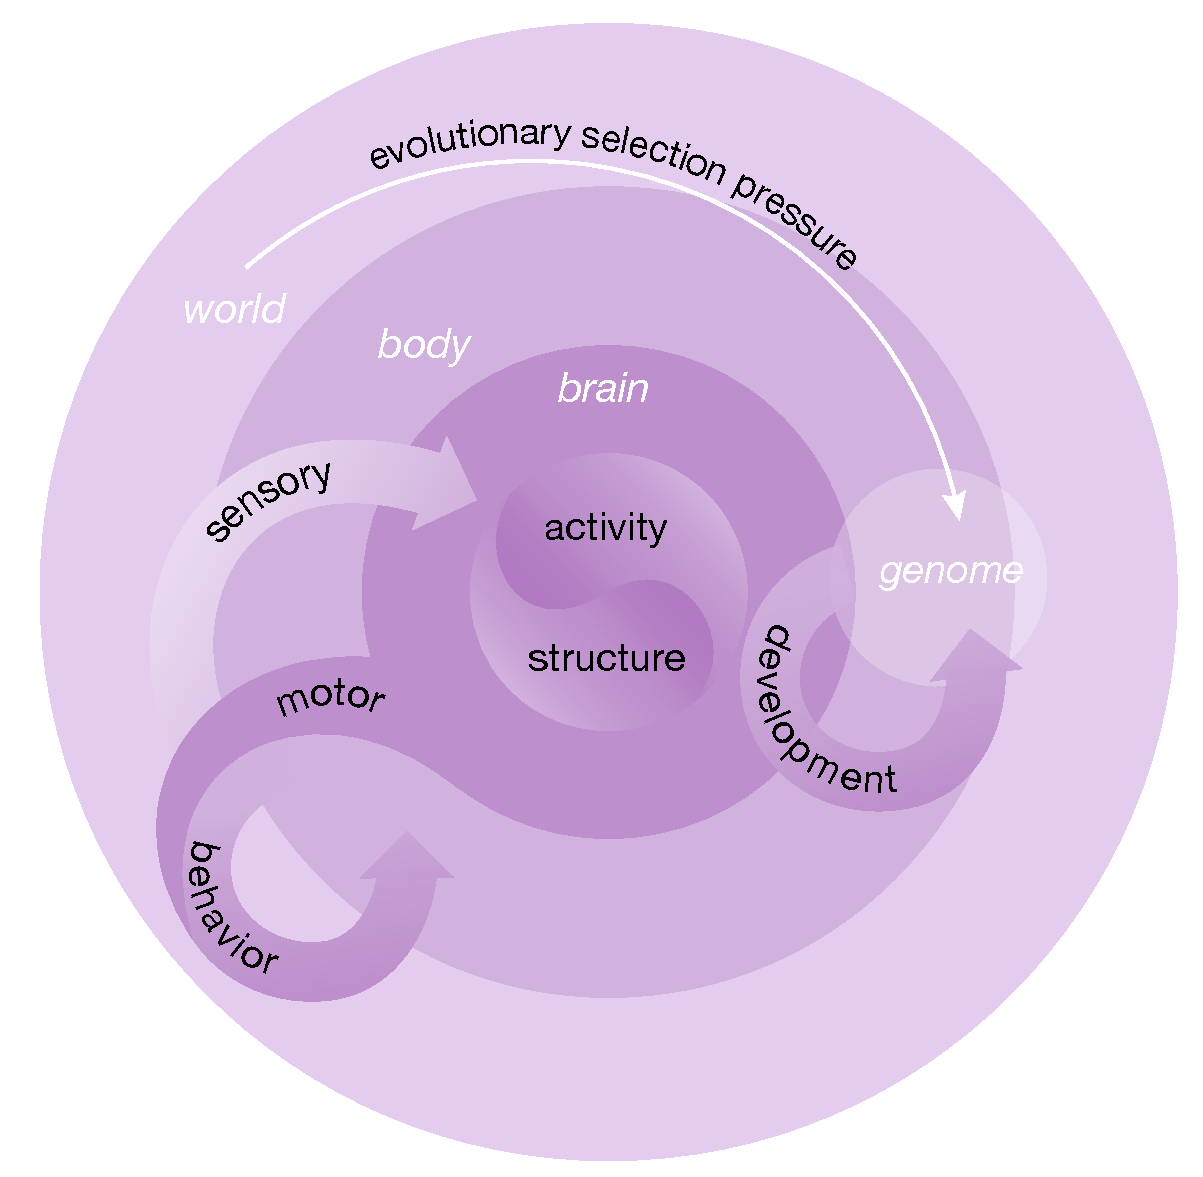
\includegraphics[width=0.5\linewidth]{figs/connectome-coding-schematic}
%	\caption{}
%	\label{f:code}
%\end{figure*}


% @BM: past "something" not maybe environment, rewrite in terms of the loops. 




\subsection{Models}





Adopting notation typical of neural coding, let $S$ denote a realized stimulus  and $R$ denote the realized response.   
We model both the stimulus and the response as random variables, denoted $\mb{S}$ and $\mb{R}$, respectively.
The neural \emph{encoding} problem is to estimate the conditional distribution of a neural response given the stimulus, $F_{R | S}$, whereas the neural \emph{decoding} problem is to estimate the distribution of the stimulus given a response, $F_{S | R}$. The joint distribution of the response and the stimulus can be written in terms of either conditional distribution, using Bayes rule: 
\begin{equation}
F_{R,S} = F_{R|S} \times F_S = F_{S| R}\times F_R.
\end{equation}

%In this review we will focus on the connectome encoding problem, $P_{R|S}$, building up from the simplest, to much more complex and structured models. 


The main assumption in connectome coding is that the information in  plasticity and development is encoded in a given set of morphological objects (for example, neurons  or gyral regions) and connections between them.
Thus, for connectome coding, we need to define some additional concepts and notation. 
Denote a network  by $\mc{G}= (\mc{V},\mc{E})$, where $\mc{V}$ is the set of nodes, and $\mc{E}$ is the set of edges,  the number of nodes is $n=|\mc{V}|$.
% , and $u \sim v$ indicates an edge between vertex $u$ and vertex $v$. 
Throughout, we will refer to the ``nodes'', which might represent neurons or regions of interest, as appropriate.
We can represent a network by an $n \times n$ adjacency matrix, $A$.   If the connectome is binary (meaning no weights on edges), than the existence of an edge between node $u$ and node $v$ is indicated by $A(u,v)=1$, otherwise, $A(u,v)=0$.  If the connectome is weighted, then $A(u,v)$ can take any real value. 
If the connectome allows self-connections (also called self-loops), then it is possible that $A(u,u)=1$ for any $u$, but otherwise not.  
 If it is undirected, then $A(u,v)=A(v,u)$ for all $(u,v)$ pairs.  
 The total number of possible edges, $n_e$, depends on whether the network is directed and whether it allows for self-loops.  If both, then $n_e=n^2$.  If neither are allowed, then $n_e = \binom{n}{2}$. 
 We will see examples of weighted and unweighted, directed and undirected networks, both with and without loops.
 
 To build  statistical models of connectomes and connectome code requires introducing the concept of random variables, as in neural coding.  Let $\mb{A}$ denote a random adjacency matrix (which is akin to the response in neural coding), and let $\mb{X}$ be  the random variable whose values denote some properties of the genome, body, and/or world. Then we can write the joint distribution of the connectome and other stuff as:
 \begin{equation}
F_{A,X} = F_{A|X} \times F_X = F_{X| A}\times F_A.
\end{equation}
For simplicity, in this review, we will focus on the connectome encoding problem, that is, determining $F_{A|X}$, which requires a prior  model $F_A$ to build on.  
 In a connectome with $n$ nodes  and  $n_2$ potential binary edges, there are $2^{n^2}$ possible different connectomes.  Note that this means that the number of possible connectomes grows at a super-exponential rate.  For example, when $n=10$, $2^{n^2}=10^{30}$, and when $n=30$, $2^{n^2}=10^{280}$!
 This is in contrast to the number of seconds  since the big bang ($\approx 10^{20}$), the number  of molecules in the universe ($\approx 10^{80}$),   the number of possible chess games ($\approx 10^{120}$), and  the number of possible go games on a $19 \times 19$ board ($\approx 10^{170}$).
 Since connectomes are fundamentally categorical objects, without further assumptions, the ``non-parametric'' connectome model would be that $\mb{A} \sim F(\bth)$, where $F$ is  a categorical distribution with parameter $\bth=(\bth_1,\ldots, \bth_{2^{n^2}})$. Clearly, $2^{n^2}$  parameters is far too many to be able to  estimate with reasonable sample sizes, even for the smallest connectomes.  Thus, connectome coding {requires} making a number of simplifying assumptions to enable empirically  useful estimates.  Below we describe several increasingly complex models of connectomes.   
  For each, we introduce the corresponding neural code.
 In a certain sense, any study of brain structure and connectivity or circuitry can be cast as a connectome coding study.

 



\section{Conclusion}

This review introduces and summarizes the basic concepts and preliminary examples of connectome coding.  An open-source  R package containing all the functions required to estimate any of the models on network data is available at \url{https://neurodata.io/} and  \url{https://github.com/neurodata/graphstats} \cite{Bridgeford2018}.

There are a  large number gaps in our knowledge and capabilities with regard to connectome coding.  Our intermediate term goal is to continue to develop theory, methods, and applications for zero-inflated, weighted, latent structure models for individuals and populations, including statistically and computationally efficient estimation and hypothesis testing in these models~\cite{Tang2017-jm}. Incorporating network, vertex, and edge attributes into this formalism is yet another future direction. 
Connectome coding therefore presents a substantial opportunity for discovery in brain sciences.

%
% \section{Comparative Connectomics}

% \subsection{ZWER}

% Even for this extremely simple set of models, it can still be interesting to compare connectomes, that is, do ``comparative connectomics''. Due to  model simplicity, we can derive uniformly most powerful two-sample tests.  Specifically,  $\pi$ is the parameter of a binomial, because there are $|\mc{E}|$ observed edges out of a possible $n_e$, and they are each independent.  Thus, Fisher's exact test can be used to test whether $\hat{\pi}$ differs from $\hat{\pi}'$.  Asymptotically, the distribution of $\hat{\pi}$ converges to a Gaussian, so a t-test is sufficient.  Similarly, $\hat{\mu}$ is the average of a large number of independent random variables, so by the central limit theorem, its distribution is asymptotically Gaussian, and thus a two-sample t-test is sufficient.  Finally, if we have both $\hat{\pi}$ and $\hat{\mu}$, then we can use Hoteling's test, which is the multivariate generalization of the t-test.  Figure~\ref{f:ie_comp} shows which connectomes are statistically significantly different from one another.

% \subsection{CIE}

% Given these estimates, it is  natural to wonder which of these models best fits the data.  Because each parameter is a binomial, we can simply apply the two-sample binomial test to check whether
% $a=b$ to compare the \mtt{PPM} to the \mtt{ER}, $a=c$ to compare the \mtt{SBM} to the \mtt{PPM}, and
%  $b=d$ to compare the \mtt{SSBM} general \mtt{SBM}.
%  We can similarly  construct  a matrix of weights, $\mu=[ \mu_{11}, \mu_{12}; \mu_{21}, \mu_{22}]$.  The MLE is available for these parameters as well, by the same reasoning.  
 

% Applying these tests to the real data yields the following results.  
% \eb{put the below results in a table?}
% For the C.~elegans, the chemical connectome yields XXX, whereas the gap junction yields XXX.  
% For the mouse connectomes, XXX.
% For  human connectomes, the p-values are XXX.  



% \subsection{Matched Graphs}

% \subsection{Unmatched Graphs}




%
%\subsubsection{Conditionally Dependent Connectomes}
%
%mixture of random graph models, a la joint embedding and omni

% \vspace{4mm}

% \noindent Many neural connectomes are dynamic. In other words, they exhibit connectivity changes over time. Time-varying graphs have become a topic of active research in recent years [?]. The simplest time-varying random graph model is an extension of the static ER random graph model previously discussed, where a time dimension is added. At every time point, each edge in the graph exists with probability p and does not exist with probability 1-p. 

% Another simple extension are random graphs that follow a Markov chain. In this model, each edge in $G_{t}$ either exists or does not exist, the choice of which depends on a binary random variable, denoted:

% \begin{align}
% \{W_{n}: n=0,...,N\}
% \end{align}

% \noindent whose state space is {0,1}. The Markov chain is characterized by the following transition probability matrix $Q$, for some choices of the birth and death rates, denoted by $p$ and $q$ respectively.

% \begin{table}[H]
% \centering
% \setlength{\extrarowheight}{7pt}
% \begin{tabular}{lll}
% \hline
%  & $W_{n+1}=0$ & $W_{n+1}=1$ \\ \hline
% $W_{n}=0$               & $1-p$ & $p$ \\
% $W_{n}=1$              & $q$ & $1-q$ \\ \hline
% \end{tabular}
% \end{table}

% Just as in the static case, the probability of an edge between neurons may be dictated by the type of each neuron. These are called dynamic stochastic block models. WILL ADD MORE HERE ABOUT DYNAMIC STOCHASTIC BLOCK MODELS.

% CAN ADD STUFF ABOUT TEMPORAL EXPONENTIAL RANDOM GRAPH MODELS IF WE WANT. COULD ALSO TALK ABOUT HMMS FOR DYNAMIC FUNCTIONAL CONNECTIVITY, BUT MAY NOT BE BEST FOR THIS PAPER? LET'S DISCUSS BEFORE I KEEP WRITING. 


%
%- given that the two have the same model, test semipar style?
%- if they do not have the same set of labeled vertices, sgm o semipar or non-par
%
%
%\section{other stuff?}
%
%- batch effects?
%- supervised joint embedding?
%- testing?
%- decoding?
%- directed? hollow? vertex attributes? edge attributes?
%
%\section*{stuff to do}
%
%\begin{itemize}
%\item R package with code that runs each example, including sampling and estimation
%\item figures
%\item refining text
%\end{itemize}


%\end{multicols}

\paragraph{Acknowledgements} 
{\small
The authors from JHU are grateful for the support  from  DARPA SIMPLEX
program through SPAWAR contract N66001-15-C-4041.
}

% \paragraph{Author Information}

% \vspace{10pt}
% {\small
%  EWB$^{1, 3, 5}$, JTV$^{1,3,5,9,17,\dagger}$: \\
% \noindent${^1}$ Johns Hopkins University.\\
% \noindent$^\dagger$ is the corresponding author: $\langle$\url{jovo@jhu.edu}$\rangle$}.


\vspace{-10pt}


\bibliographystyle{unsrtnat}
\begin{spacing}{0.3}
{\footnotesize  \bibliography{statconn}}
\end{spacing}

\clearpage
\subsection*{Highlights} 

\begin{enumerate} 
\item Connectome coding is analagous to, although more complex than, neural coding. 
\item Latent structure models impose parametric and geometric requirements on networks. 
\item Population models can estimate properties jointly from many disparate connectomes.
\end{enumerate}


\section*{Annotated References}

\subsection*{Special Interest}

\begin{enumerate}
    \item \cite{Kiar2018-bo} provides the largest open-access repository of human connectomes.
    \item \cite{Eichler2017-yi} is one of the  most recent and comprehensive characterizations of a connectome.
    \item \cite{Van_Dam2017-cv} describes a new approach to understand psychiatric disorders using connectomics.
\end{enumerate}

\subsection*{Outstanding Interest}

\begin{enumerate}
    \item \cite{Athreya2018-ks} describes the  latent structure models that impose parametric and geometric requirements on networks.
    \item \cite{Levin2017-ec} describes the omnibus methodology for inference on populations of networks.
    \item \cite{Hodge2018-dr} describes the first large scale cell atlas
\end{enumerate}

\clearpage
\appendix

\renewcommand\thesection{Appendix~\Alph{section}}
\renewcommand{\thefigure}{S\arabic{figure}}
\setcounter{figure}{0}



%\theendnotes

\end{document}
